
\newif\ifcameraready
\camerareadyfalse
\providecommand{\OpenHandsArtifactURL}{https://github.com/vals-ai/VibeCodeBench-Openhands-Scaffold}
\providecommand{\VCBTrajectoriesURL}{https://github.com/vals-ai/vibe-code-bench-paper-artifacts}
\providecommand{\Description}[1]{}


\subsection*{Source Note}
This section is derived from VibeCodeBench. Alex contributed but is not first
author, so the material is kept in blue and should be rewritten before final
submission. The section includes only the field-shaping point needed for this
chapter.

\subsection{Full Web-Application Generation}
VibeCodeBench is included in this chapter because it turns ``build a complete
application from scratch'' into an evaluation target. Existing code benchmarks
often measure isolated function synthesis, competitive-programming solutions,
or bug fixes inside an existing repository. VibeCodeBench instead asks whether
a model can start from a natural-language product specification and produce a
runnable web application.

That changes the evaluation object. A generated application must satisfy
user-visible workflows, not merely pass local unit tests. The model has to
create a multi-file project, wire together frontend and backend behavior, handle
state and persistence, and support workflows that a browser-based evaluator can
execute end to end. This is closer to the way non-technical users imagine
``vibe coding'': describing the product they want and receiving a usable
application.

\subsection{Browser-Based Workflow Evaluation}
The benchmark uses application specifications paired with browser workflows.
Each workflow is decomposed into substeps, and an autonomous browser evaluator
tests the deployed application through the UI. This makes the metric
implementation-agnostic: a model can choose its own internal structure as long
as the user-visible behavior satisfies the specification.

This measurement choice matters. Unit tests are effective for functions and
some repository tasks, but they do not naturally capture whether a user can
sign in, create an object, navigate to the right page, trigger an email, or
complete a multi-step transaction. Browser workflows make those product-level
behaviors measurable.

\begin{figure}[tbp]
  \centering
  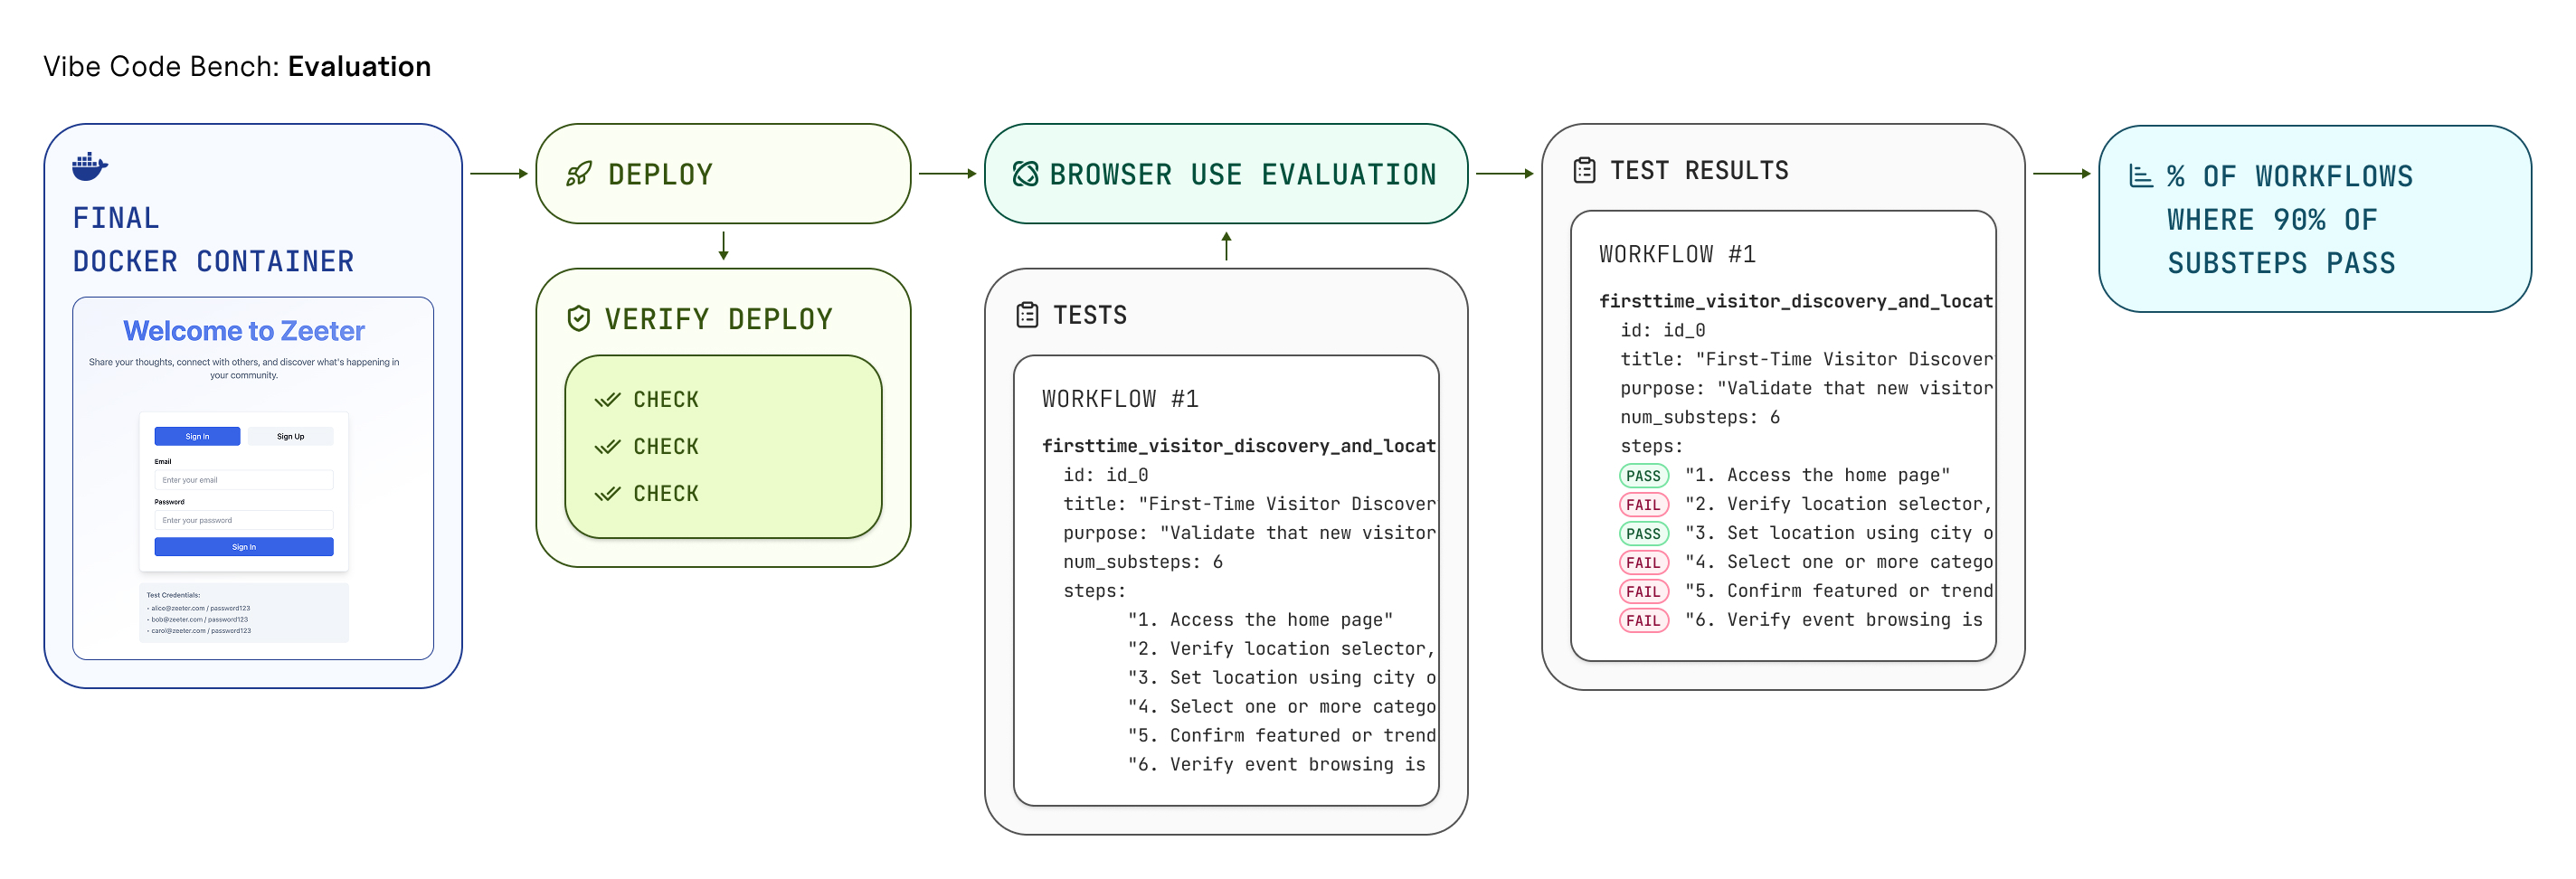
\includegraphics[width=0.85\linewidth]{evaluation_schematic.jpg}
  \caption{VibeCodeBench evaluates generated applications through browser-based
  workflows, making end-to-end product behavior the object of measurement.}
  \label{fig:vibecodebench-eval-thesis}
\end{figure}

\subsection{Why This Shapes System Building}
The field-shaping point is that once full-application generation is measured,
models and agents can be compared on end-to-end product behavior rather than
only local code correctness. This pushes systems toward capabilities that
single-function benchmarks do not require: project setup, UI consistency,
database wiring, authentication, integration with external services, and
self-testing in the browser.

The paper also reports that model behavior during generation matters. In
particular, self-testing with a browser is associated with stronger final
performance. This is a useful example of measurement shaping what gets built:
if the benchmark evaluates deployed app behavior, then agents have an incentive
to test their own apps in the same medium users will use.

\subsection{Thesis Takeaway}
VibeCodeBench illustrates the chapter's claim that metrics define engineering
targets. When the metric is browser workflow completion, the system must become
more than a code generator. It must become an application builder that can
construct, run, inspect, and revise a working product.
